\documentclass{standalone}
\usepackage{tikz}

\begin{document}

  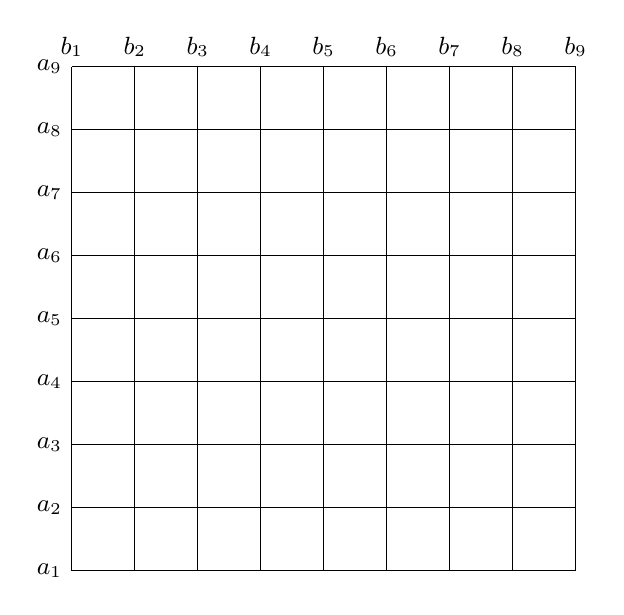
\begin{tikzpicture}[scale= 0.4,>=latex]
    \foreach \n in {1,...,9}{
      \draw (2*\n-2,0)--++(0,16)node[above]{\small $b_{\n}$} (0,2*\n-2)node[left]{\small $a_{\n}$}--++(16,0);
    }
  \end{tikzpicture}
  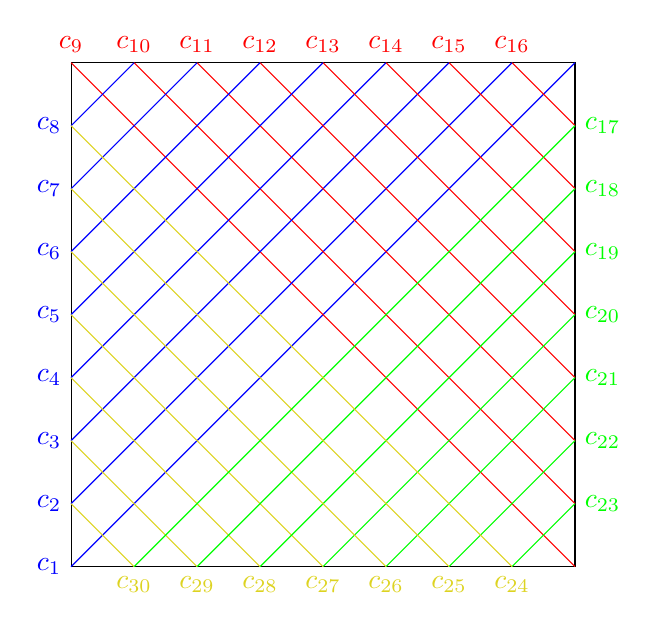
\begin{tikzpicture}[scale=0.8]
    \draw (0,0) rectangle (8,8);
		\foreach \n in {1,...,8} \node [left,blue] at (0,\n-1) {\(c_{\n}\)};
		\foreach \n in {9,...,16} \node [above,red] at (\n-9,8) {\(c_{\n}\)};
		\foreach \n in {17,...,23} \node [right,green] at (8,24-\n) {\(c_{\n}\)};
		\foreach \n in {24,...,30} \node [below,yellow!85!black] at (31-\n,0) {\(c_{\n}\)};
    \foreach \n in {0,...,8}{
			\draw [blue] (0,\n) -- (8-\n,8);
			\draw [red] (\n,8) -- (8,\n);
    }
		\foreach \n in {1,...,7} {
			\draw [green] (8,\n) -- (8-\n,0);
			\draw [yellow!85!black] (\n,0) -- (0,\n);
		}
  \end{tikzpicture}

\end{document}
